%%% compile it with pdflatex
\documentclass[a4paper]{article}
\usepackage[T1]{fontenc}
\usepackage[utf8]{inputenc}
\usepackage{lmodern}
\usepackage{fancybox}
\usepackage{graphicx}
\usepackage{tabularx}
\usepackage{amssymb}
\usepackage{amsmath}

\begin{document}

\title{A Multi-Agent System for\\ playing Briscola Chiamata}
 
\author{Beltran Borja Fiz, Fabrizio De Santis, Marcos Gabarda\\
\small \texttt{\{beltran.borja.fiz, fabrizio.de.santis, marcos.gabarda\}@est.fib.upc.edu}\\
\\
Multi-Agent Systems Course\\
Master in Artificial Intelligence\\
Universitat Polit\`ecnica de Catalunya}
\date{\today}

\newenvironment{fminipage}%
  {\begin{Sbox}\begin{minipage}}%
  {\end{minipage}\end{Sbox}\fbox{\TheSbox}}


\maketitle

\tableofcontents

\newpage

\section{Introduction}\label{sec:intro}

2-APL stands for Abstract Agent Programming Language , and is developed at the University of Utrecht as an academic tool for developing intelligent multi-agent systems. With its unique feature of integrating a declarative and an imperative style programming and the ability to use the JADE platform, 2APL is a resourceful environment to program in.

In a previous Paper we described the features of 2APL, along with a more formal description of the language. Its tools were presented and a few examples were showcased to see some agents in action.The aim of this Paper is to present our own prototype of a 2APL multiagent system to model the card game of Briscola Chiamata. In particular, we present in section 2 a description of the game . In the next sections we follow the Prometheus design methodology to create our system. We display the built prototype in Section 6 and w e conclude the paper in section 7 with some remarks, related works and conclusions on the overall success of the prototype.

There are many features that make Briscola Chiamata an ideal game to model with a multiagent system. The way the game works forces the developer to give agents cooperation, while at the same time being competitive; they have to be reactive, but also proactive; finally they need to also be autonomous and social.

Cooperation in Briscola Chiamata is a double-edge sword, since if you choose the wrong player to cooperate with, you will be cause your own defeat. On the other hand, a successful cooperation will most of the time ensure a safe victory. This risk in choosing who to trust and cooperate with is what makes the game exciting for humans, and hard for agents.Competition is divided into two types, an individual agent competing to win the game, and a team of agents, trying to compete against the opposite team.

Reactivity is an obvious requirement in any group game; when it is your turn to play, you have to play. In Briscola Chiamata however a Proactivity is also required since players need to bid only if they desire and the turns are non strict, i.e: a player can decide to play outside his turn. This freedom of the game needs to be given to the agents.

The social factor comes from the fact that players have to interact with each other in order to advance the game. The bidding system each round of the game and the fact that teams are created without the agents knowing who they are partners with creates the necessity for communication between them in order to try and determine who this partner is. Having agents change status from partner to opponent between rounds makes a dynamic social multiagent system which is worth studying.


\section{Game Description}

\emph{Briscola Chiamata} is the five-player version of \emph{Briscola}. Every player is dealt eight cards, so that no cards remain undealt. Then, each player, starting from the dealer's right\footnote{If the dealer is not a player, then starting from the declearer's right} and proceeding counter-clockwise, bids in an auction to declare how many points they will score. A player may pass, and hence cannot bid again in that game. The bid represents the number of points that player believes he is capable of accumulating. Bidding continues until all but one player have passed in a round. This remaining player has then "won the bid" and therefore gets to declare the Briscola. The declarer also declares a specific Briscola card (example, the ``Ace of Cups'' if Cups was the declared Briscola) and the holder of this card is then determined to be the declarer's partner. Logically, the declarer would declare the highest Briscola card he does not already hold in the hopes of creating the strongest combined hand between him and his partner.
The remaining three players are partnered with each other, without their knowledge. Each player, other than the declarer's partner, acts independently, until it is clear which players are partners. Infrequently, the declarer may declare a Briscola card he already holds (if he feels he has a very strong hand), in which case the other four players are partenered against him.
Game strategy is often devised to determine which player is partnered with the declarer, whereas the declarer's partner may devise ruses and decoy strategies to fool the other players, such as not taking a trick, or playing points on a trick that will be won by an opponent.

\paragraph{Scoring}

Each player collects tricks as per the regular version of the game, and counts points collected similarly. Partners, which are known by the end of the game, then combine their points. Game points are assigned as follows: if the declarer and partner accumulate card points greater than or equal to the points that were declared after the bidding process, then the declarer earns two game points, the partner earns one game point and the other players each lose one game point. If the declarer and partner accumulate fewer card points than declared, then  the declarer loses two game points, the partner loses one game point and the other players each earn one game point. These points are accumulated after every game. The grand winner is the player with the most points at the end of the last match. Note that if the declarer calls a Briscola he holds, then the declarer will win or lose four points, and every other player will win or lose one point.

\section{System Specification}\label{sec:sysspec} 

In this phase, actors (human or software) expected to interact with the system, are identified, along with the interface to the system in terms of actions and percepts; system goals are elaborated, and scenarios described in terms of sequences of steps are developed. Roles encompassing small chunks of functionality (identified by goals, percepts and actions) are described and captured.

\subsection{Analysis Overview Diagram}

The analysis overview diagram is designed to show the interactions between the system and the environment. At this abstract level it is necessary to identify the actors, scenarios, percepts and actions involved in the system. This consists of a two step process. Firstly, we identify the actors and the scenarios they participate in with the system. Secondly, we identify and define the actions and percepts between the actors and the system.

The actors are all the people or external systems associated with the system. The scenarios are the processes which the system uses to handle the percepts and produce the actions. The percepts are all the types information which come into the system from the environment. The actions are everything that is sent from the system to the environment.

%Specify key external actors that will use the system, and key scenarios they will be involved in.
%Link the actors to the scenarios they are involved in, using percepts and actions. Percepts are signals from actor to system. Actions are responses from the system, possibly directed towards a particular actor. This diagram can be used very freely to sketch a design of the system.

Actors:
\begin{itemize}
  \item User: user of the system
\end{itemize}

Scenarios:
\begin{itemize}
  \item Start the game scenario: join requests are received. Two options are possible: the request is accepted or queued. A message is then sent back acknowledging the request.
  \item Dealing scenario: if there are 5 players subscribed in the system, then a card dealer is chosen that shuffle the deck and deal the cards to all the players.
  \item Bidding scenario: once the dealing is over, players can start bidding in turn. The player who wins the bid, must declare the Briscola card. If nobody bids, then the game has to be restarted.
  \item Play the Game scenario: once the Briscola card has been declared, the players start playing. The teams setting is unknown to all the players until the Briscola card is played. The players have to update their beliefs about teams setting each time a card is played. Of course, cheating is part of the game. Communication (sign exchange) among players is allowed to exchange information about players and cards. After each hand, points are counted.
  \item End the game scenario: once the winner team is declared, scoring is updated and players are released from the system.
\end{itemize}

Inputs/outputs (percepts/actions)
\begin{table}[htp]
  \begin{tabular}{|l|l|}	
    Join request	& Subscribe user and manage request (the request has been accepted or queued) \\
    \hline
    5 players in the system	& Choose the card dealer and start shuffling and dealing cards to the players \\
    \hline
    Dealing is over	& Start bidding in turn \\
    \hline
    Bidding is over	& Declare the Briscola card \\ 
    \hline
    Briscola declared	& Start playing in turn \\
    \hline
    Card played	& Update internal beliefs about teams setting \\
    \hline
    Message from other players (Sign exchange)	& Update internal beliefs about teams setting \\
    \hline
    The hand is over	& Count points \\
    \hline
    The game is over	& Declare the winner \\
    \hline
    Winner declared	 & Update the system scoring \\
    \hline
    System scoring updated	& Release the agents from the system \\
    \hline
  \end{tabular}
\end{table}

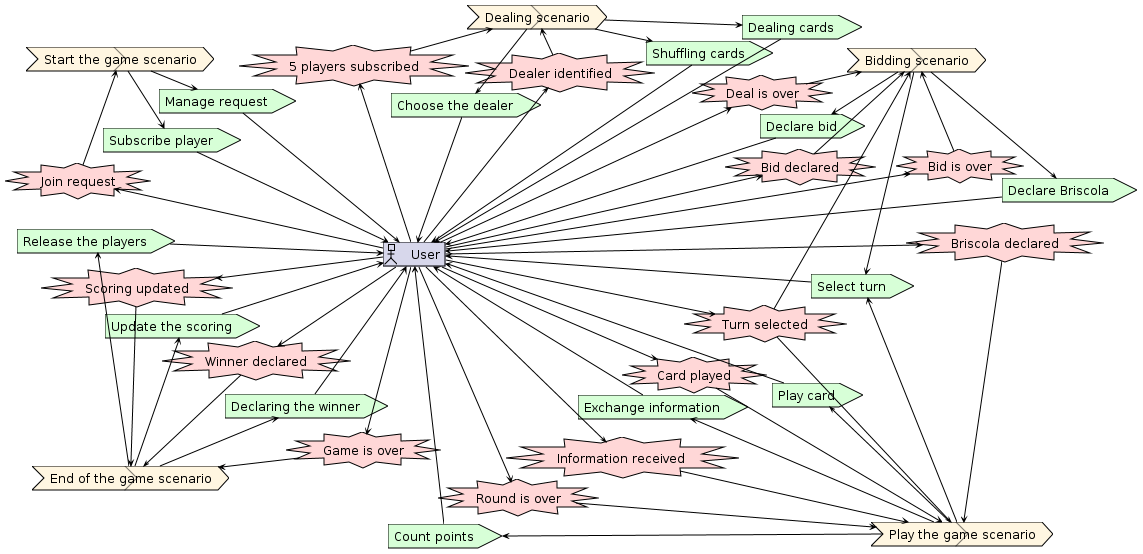
\includegraphics[keepaspectratio,scale=0.3]{pdt/images/system_specification/analysis_overview.png}

\subsection{Scenarios Diagram}

Scenarios are an example of the dynamics, the process of how something can happen. Conversely, the goal hierarchy is a static representation  - it tries to break down all the high level goals into subgoals. Each scenario must be associated with some goal, that represents what that scenario is trying to achieve. 

\begin{enumerate}
  \item Start the game scenario
  \begin{itemize}
    \item Register players and inform them to wait if there are less than 5 players registered
    \item Queue players if there are already 5 players registered
  \end{itemize}
  \item Dealing scenario
  \begin{itemize}
    \item Choose the card dealer
    \item Shuffle the deck
    \item Deal cards
  \end{itemize}
  \item Bidding scenario
  \begin{itemize}
    \item Start bidding in turn until the highest bid is established
    \item Declare the Briscola card
  \end{itemize}
  \item Play the Game scenario
  \begin{itemize}
      \item Play cards in turn
      \item Collect points for each hand
  \end{itemize}
  \item End the game scenario
  \begin{itemize}
    \item Count points
    \item Declare the winner
    \item Release the players
  \end{itemize}
\end{enumerate}

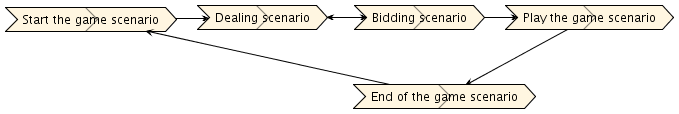
\includegraphics[keepaspectratio,scale=0.3]{pdt/images/system_specification/scenarios.png}

\subsection{Goals Diagram}

The goal overview diagram is a directed acyclic graph of all goals in the system. Sub-goals can be generated by asking ``how will the system accomplish this goal'' Parent goals can be generated by asking ``why does the system accomplish this goal'' .

  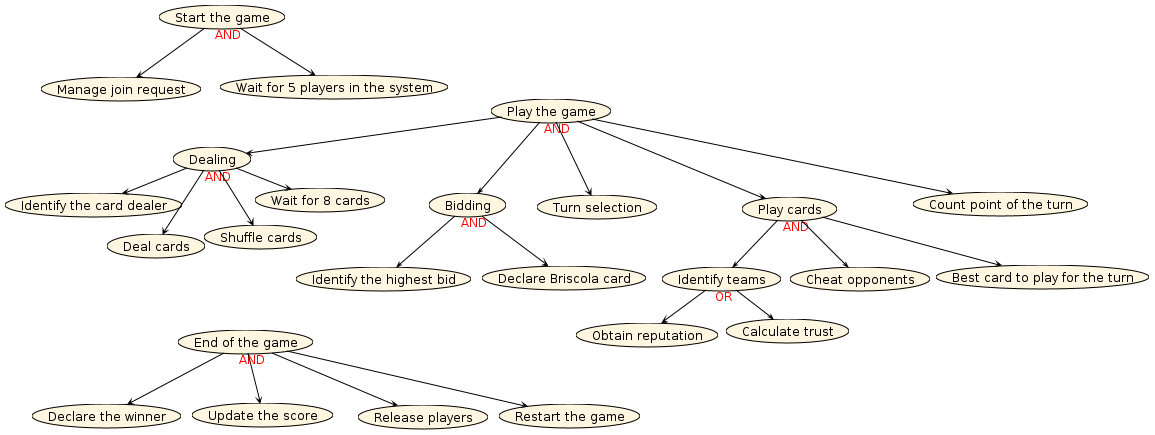
\includegraphics[keepaspectratio,scale=0.3]{pdt/images/system_specification/goal_overview.png}

\subsection{System Roles Diagram}
The next stage of the process is to group similar goals together into roles. Each role should be limited in scope, and be able to be described fully be 1-2 sentences. Grouping is done using the System Roles diagram. In a system roles diagram, we group different goals, percepts and actions under roles. This helps in further modularizing the system. The input is represented as a percept and the output as an action.

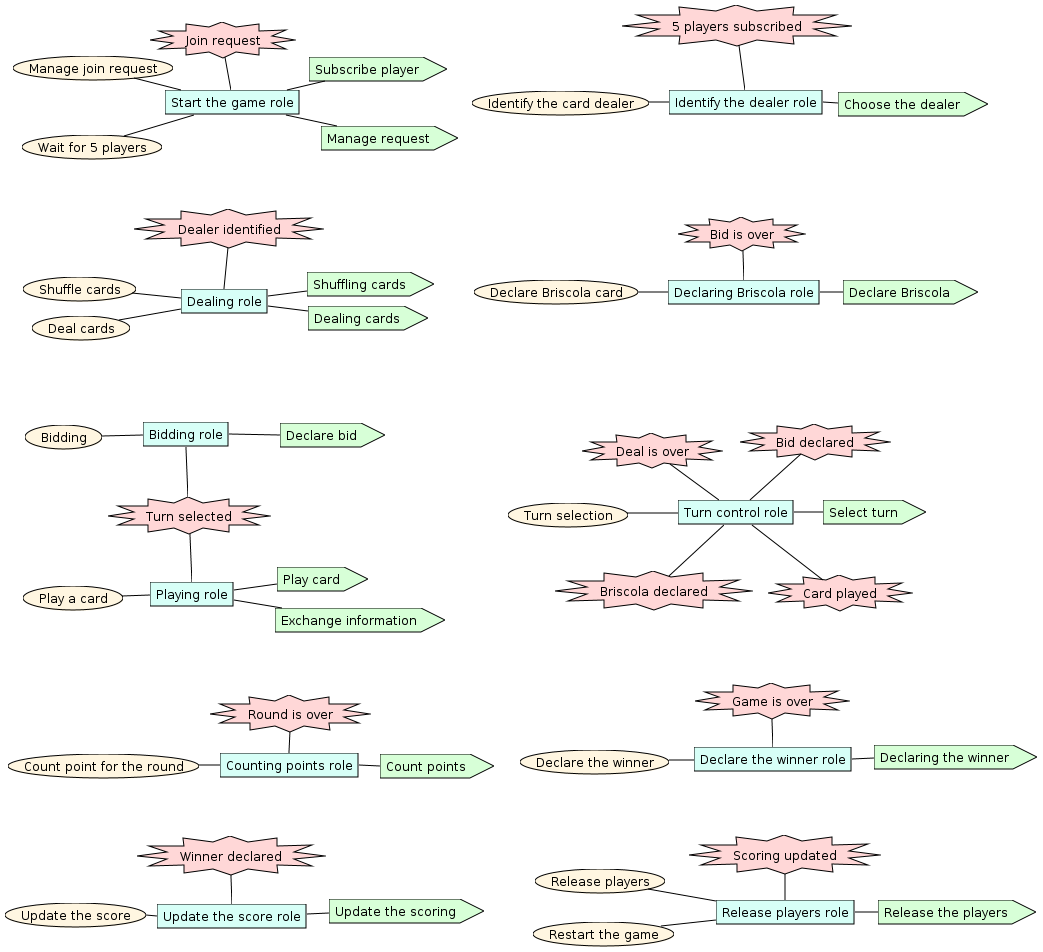
\includegraphics[keepaspectratio,scale=0.3]{pdt/images/system_specification/system_roles.png}

\section{High-level (Architectural) Design}\label{sec:highdesign}

In this phase, the agent types that will exist in the system are defined by combining roles, the overall structure of the system is described using a system overview diagram, and interaction protocols are used to capture the dynamics of the system in terms of legal message sequences.

\subsection{Data Coupling Diagram}

The roles that were formed in the last step of the previous phase are linked to data that has been identified as necessary for performing that role. In the data-coupling diagram you can see all roles and data types in the system.

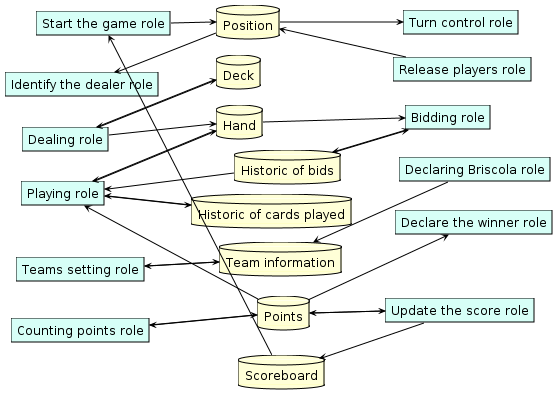
\includegraphics[keepaspectratio,scale=0.3]{pdt/images/architectural_design/data_coupling.png}

\subsection{Agent-Role Grouping Diagram}

In this diagram we group the roles into agent types. Decisions regarding how to group depend on role similarity, as well as analysis of data usage. The agent-role coupling diagram shows the group of roles that come under an agent.

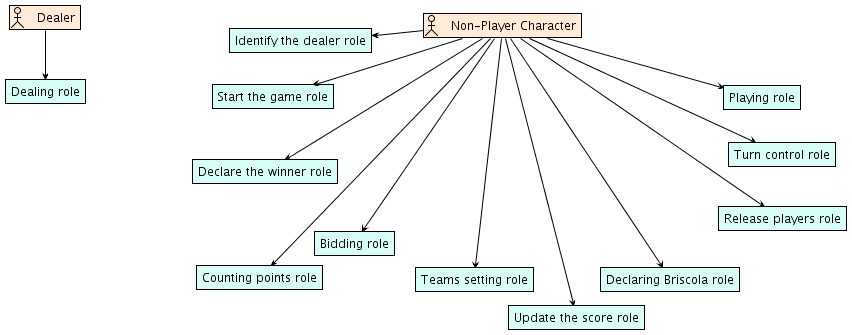
\includegraphics[keepaspectratio,scale=0.3]{pdt/images/architectural_design/aget-role_grouping.png}

\subsection{Agent Acquaintance Diagram}

In the agent acquaintance diagram you can see all agents within the system and which agents interact.

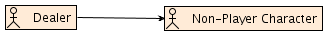
\includegraphics[keepaspectratio,scale=0.3]{pdt/images/architectural_design/agent_acquaintance.png}

\subsection{System overview Diagram}

In the system overview diagram you can see all agents in the system, along with their interface and interactions. This diagram is the central diagram of the entire system design.

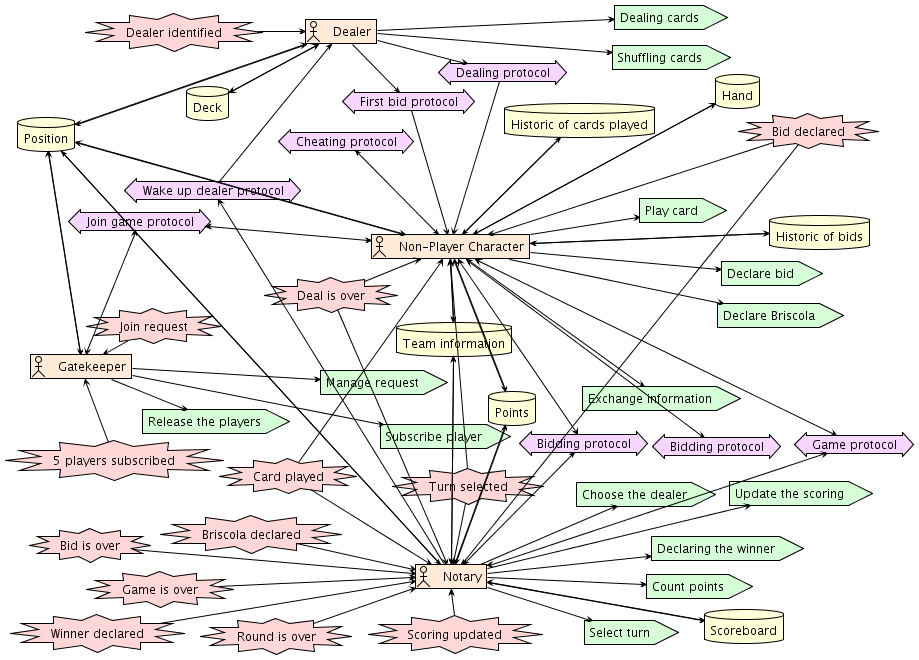
\includegraphics[keepaspectratio,scale=0.3]{pdt/images/architectural_design/system_overview.png}

\section{Detailed Design}\label{sec:detaildesign}

n this phase, the internals of each agent are developed in terms of capabilities, events, plans and data. Detailed Design is done at the level of individual agents.

\subsection{Agent Overview Diagram}
The agent overview diagram shows the internals of an agent. There is one agent overview diagram for every agent in the system. In the detailed design, much finer details of the system are established. The messages used to communicate between the agents are decided upon. If the roles within an agent grow very large, they are grouped into capabilities. As in the system overview diagram entities can be inserted or removed and edges can be reated or deleted.

\subsection{Capability Overview Diagram}
In the capability overview diagram you can see the direct internal of a capability. This diagram allows you to specify the internals of a capability in terms of plans, or sub-capabilities and messages between them. Data internal to the capability can also be specified.

\section{Prototype}\label{sec:proto} 

Description. Excerpt from the code.

\section{Conclusion}\label{sec:concl} 

What's wrong with 2APL?

No security mechanisms, No documentation like a manual or of examples (only short example provided with the platform). Not all the constructs available are documented (e.g. random() or print())

If an agent requires an action not related with changing its mental state, it has to be done through the environment. It would be nice to have agents in which part of its executing plan will consist of running some classification algorithm or some numerical method which is only owned by the agent and so it could be encapsulated in its program.

The platform is well done, but it's still a tool for research

\section{Bibliography}
\nocite{*}
\bibliographystyle{plain}
\bibliography{bc-doc}

\end{document}
